\documentclass[12pt,a4paper]{article}

% Packages
\usepackage[margin=1in]{geometry}
\usepackage{setspace}
\usepackage{graphicx}
\usepackage{titlesec}
\usepackage{xcolor}
\usepackage{hyperref}
\usepackage{float}

% Line spacing
\onehalfspacing

% Hyperlink setup
\hypersetup{
    colorlinks=true,
    linkcolor=blue,
    urlcolor=blue
}

% Section formatting
\titleformat{\section}
{\large\bfseries}
{}
{0em}
{}

\begin{document}

%------------------------------------------------
% TITLE / INFORMATION
%------------------------------------------------

\begin{center}
    {\LARGE \textbf{HCI \& COMPUTER GRAPHICS}}\\[0.3cm]
    {\Large \textbf{ASSIGNMENT NO 1}}\\[0.6cm]
\end{center}

\noindent
\textbf{Name:} AHTESHAM ALAM\\[0.2cm]
\textbf{Roll No:} 2K24/CSE/22\\[0.2cm]
\textbf{Subject:} HCI \& COMPUTER GRAPHICS\\[0.2cm]
\textbf{Class:} 3RD YEAR CS (PE)\\[0.2cm]
\textbf{Submitted To:} SIR RAJESH KUMAR

\vspace{0.4cm}

%------------------------------------------------
% IMAGE 1
%------------------------------------------------

\begin{figure}[H]
    \centering
    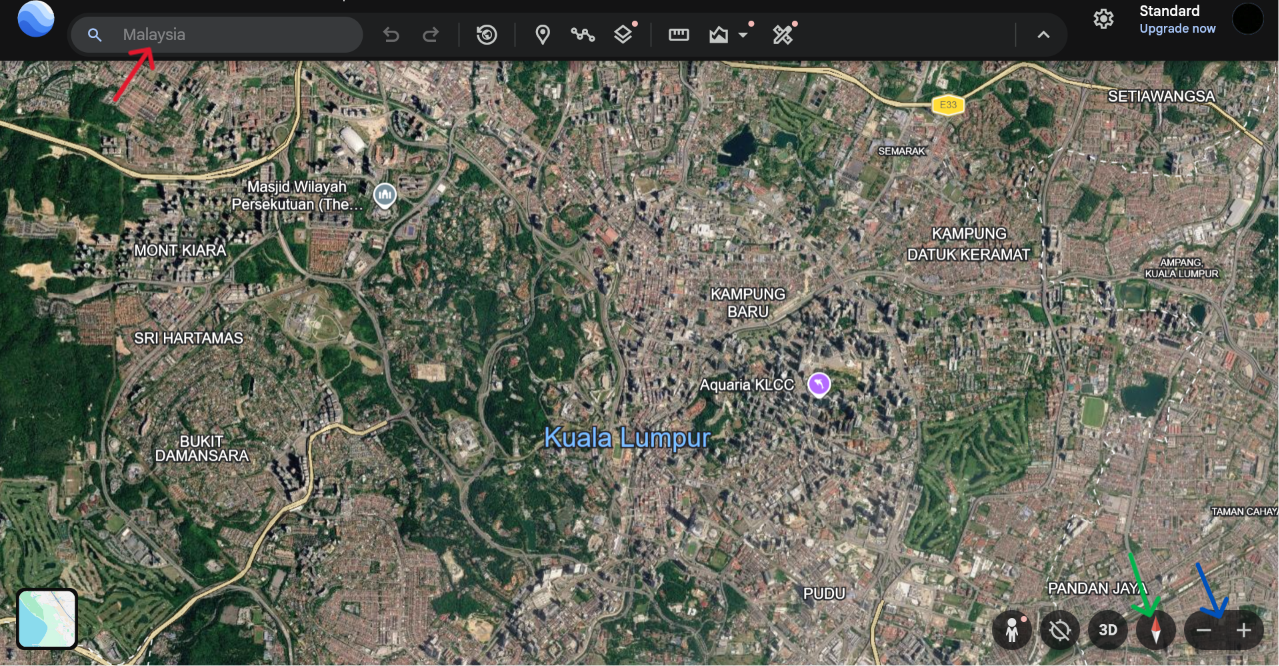
\includegraphics[width=0.90\textwidth]{Screenshot 2026-09-08 093757.png}
\end{figure}

\vspace{0.1cm}

%------------------------------------------------
% GOOGLE EARTH FEATURES
%------------------------------------------------

\noindent
\textbf{Search Bar:}
The Search Bar in Google Earth is used to search for and quickly locate
specific places, addresses, landmarks, or locations on the Earth.

\vspace{0.3cm}

\noindent
\textbf{Navigation Bar:}
The Navigation Control is used to move, rotate, tilt, zoom in, and zoom
out of the map to explore different locations and views.

\vspace{0.3cm}

\noindent
\textbf{Zoom Controls:}
The Zoom Control in Google Earth is used to zoom in and zoom out to view
a location more closely or from a wider area.

\newpage

%------------------------------------------------
% IMAGE 2
%------------------------------------------------

\begin{figure}[H]
    \centering
    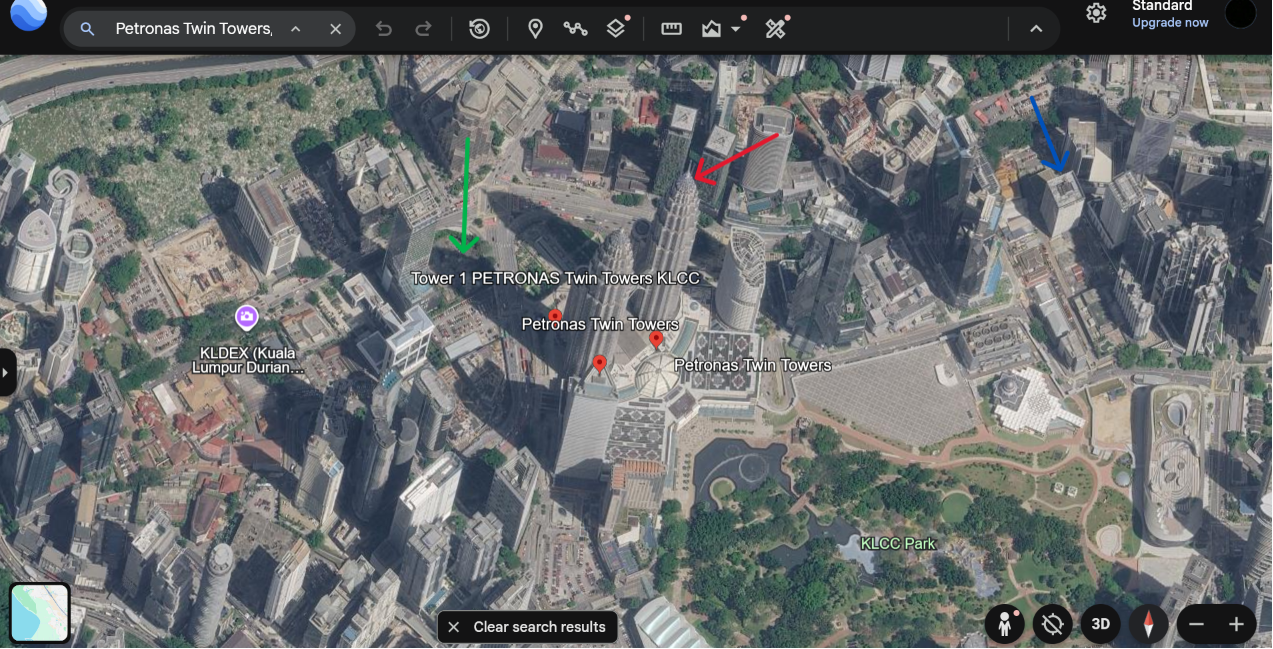
\includegraphics[width=0.90\textwidth]{Screenshot 2026-09-08 103740(2).png}
\end{figure}

\vspace{0.1cm}

\noindent
\textbf{3D Geometry:}
The 3D Geometry is used to display buildings and structures with
realistic height, shape, and depth for a three-dimensional view.

\vspace{0.3cm}

\noindent
\textbf{Shadows (Light Source):}
The Shadow (Light Source) is used to show the direction and position of
sunlight by displaying shadows cast by buildings and other objects.

\vspace{0.3cm}

\noindent
\textbf{Texture Mapping:}
The Texture Mapping in Google Earth is used to apply realistic images and
surface details to 3D buildings, roads, and other objects.

\newpage

%------------------------------------------------
% QUESTIONS AND ANSWERS
%------------------------------------------------

\section*{Question No 1}

\textbf{How does the Computer Graphics quality (e.g., realistic lighting
or 3D view) help or hinder the user's ability to interact with the software?}

\vspace{0.2cm}

\textbf{Answer:}

High-quality computer graphics make software more interactive and easier
to use. Features such as realistic lighting, shadows, textures, and 3D
views help users recognize buildings, streets, and landmarks more easily.
They also make it easier to explore places from different angles and
understand the surroundings.

\vspace{0.7cm}

%------------------------------------------------

\section*{Question No 2}

\textbf{What is one simple HCI change you would make to improve the user
interface?}

\vspace{0.2cm}

\textbf{Answer:}

One simple HCI change I would make is to use clear and easy to understand
icons with short labels or tooltips. This would help users understand each
feature more easily and make the interface more user-friendly, especially
for new users.

\end{document}
